
% Chapter 2 File

\chapter{Dissertation or Thesis Manuscript Preparation}
\label{chapter2}

\section{Sample Title Page}

Use the format below, making allowance for the left margin of 1.5 inches in centering the print. The date shown (month and year only) should reflect when the dissertation or thesis was approved. This will protect the candidate in the event an intellectual property issue related to presentation of information or date of submission should arise. A sample title page template is as shown in figure \ref{title_page}.

\begin{figure}[H]
\begin{center}
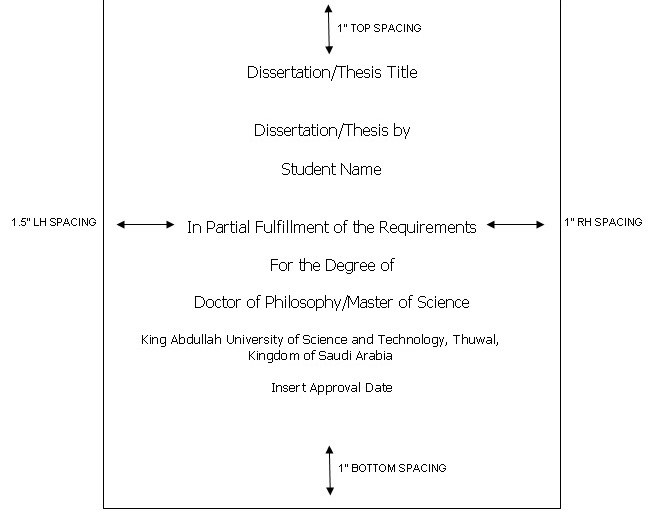
\includegraphics[scale=0.85]{Title_Page.jpg}
\caption{Sample Title Page Template \cite{guidelines}.}
\label{title_page}
\end{center}
\end{figure}

\section{Thesis Title Guidelines}

Dissertations or Theses are valuable resources for scholars that should be easily retrievable. Modern retrieval systems generally use the words in the title to locate a document. Search engines use the words in the title, and sometimes other descriptive words, to locate works. It is essential that the title be an accurate and meaningful description of the content and that obscure references be avoided. Please use these guidelines when formulating a dissertation or thesis title:

\subsection{Case}

The first and last words and all nouns, pronouns, adjectives, verbs and adverbs (if, because, as, that, etc.) are capitalized. Articles (a, an, the), coordinating conjunctions (and, but, or, for, nor), and prepositions, regardless of length, are lowercased unless they are the first or last word of the title or subtitle. Acronyms should be used sparingly throughout and they should be set in full capitals.

Examples:

\begin{itemize}
\item Solar and Wind Power
\item Engineering Technology for Developing Countries: Best Practices as Predictors of Success.
\item A Comparison of Scientific Methodologies for Determining Achievement in Graduate School Research.

\end{itemize}

\subsection{Hyphenation}

Consult a dictionary as to whether a word is hyphenated. In general words beginning with prefixes co, non, post, or re are not hyphenated unless there is a possibility of confusion (co-op, post-master's) or the root word begins with a capital letter (post-Renaissance). Hyphenate words beginning with the prefix self. Hyphenate compounds used as adjectives (decision-making) but not as nouns (decision maker). Part-time is always hyphenated. When more than one prefix is joined to a base word, hyphenate the prefixes standing alone (micro - and macroeconomics). Do not hyphenate fundraising, freelance, yearlong or health care.

Example:

\begin{itemize}
\item Important Advances in Nonlinear Equations in the Twentieth Century (Instead of: Important Advances in Non-linear Equations in the 20th Century)

\end{itemize}

\subsection{Spelling and Grammar}

Dissertation or thesis titles should be spell-checked and dictionary spelling of words should be used.  Use "and" rather than "\&", and spell out names of centuries and other numbers.

Example:

\begin{itemize}
\item The Twentieth Century Scientific Method in Perspective.

\end{itemize}

\subsection{Special Characters}

No special characters should appear in the dissertation or thesis title.  Terms or phrases that include special characters should instead be written out.  When possible, use word substitutes for formulas, symbols, superscripts, Greek letters, etc., which do not appear on most computer keyboards and would render your title unsearchable.

Example:

\begin{itemize}
\item Hybrid MPI-CUDA Strategies for GPU-based Computational Science and
Engineering Applications on Millions of Cores (instead of Hybrid
MPI-CUDA Strategies for GPU-based CS\&E Applications on 10**6 Cores).

\end{itemize}

\subsection{Italicization}

Italics should only be used in dissertation or thesis titles when referring to the title of a published work, foreign language words, gene names, scientific names as appropriate or other words that are usually italicized.

Example:

\begin{itemize}
\item Techniques in Pseudomonas Aeruginosa Biofilus Biology

\end{itemize}

\subsection{Apostrophes}

Do not use to form plurals (it should be 1980s, not 1980's) unless it would be confusing without (thus A's B's, not As and Bs; p's, not ps).  Possessives of singular nouns ending in s are formed by adding s (e.g., Harris's cat).

\section{Signature Approvals Page}

The signature approvals page must contain original signatures verifying that the dissertation or thesis and their contents have been examined and approved by the committee members. It should only contain the signatures of the certifying members of the dissertation or thesis examination committee.

The student's name as recorded by KAUST also appears on the signature approvals page. The name should be the same as that which appears on the title page and copyrght page (if the copyright is being registered). The name of each signing committee member should be typed. No titles or degree designations should be used (no Professor, no PhD, etc.). On the signature page, the title Committee Chair or Co-Chair follows each Chair's name. The student should adjust the spacing between listed names according to how many committee members there are.  There is no required order for the names of the committee members except the name of the Chair (or Co-Chairs), which appears as the last names(s) on the page. Signatures should be in black ink. The date at the bottom of the page is the year in which the degree is awarded and is the same as the year on the title page.

The signature page is always page 2 of the manuscript, and is the first page on which a number appears. Every page after this page is numbered.

The \underline{\textbf{signature approvals page is a mandatory part}} of the dissertation or thesis submission process.

\section{Sample Copyright Page}

This is an example of the copyright page, which is optional but must follow the signature approvals page and, if included, would be numbered page 3 at the top.  

If you wish to give users the right to copy and distribute your work provided they give you credit, such as via a Creative Commons license (http://creativecommons.org/\\choose/), you may insert the relevant notice following your copyright notice (e.g., "This work is licensed under a Creative Commons Attribution 3.0 Unreported License (http://creativecommons.org/licenses/by/3.0/)."

NOTE: The year on the copyright page must be the same as the year that the author received his/her dissertation or thesis approval.

Use the same margins as the title page. The copyright page template can be seen in figure \ref{copyright_page}.

\begin{figure}[H]
\begin{center}
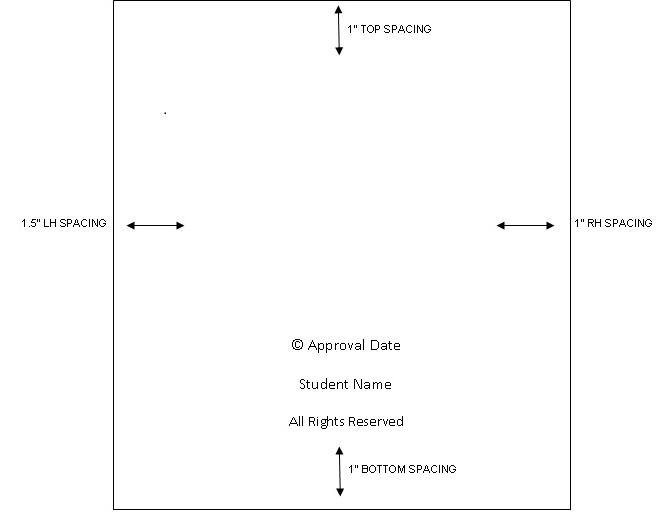
\includegraphics[scale=0.85]{Copyright_Page.jpg}
\caption{Copyright Page Template \cite{guidelines}.}
\label{copyright_page}
\end{center}
\end{figure}

% Copyright 2010 Imran Shafique Ansari
% Contact Email: imran.ansari@kaust.edu.sa
% Contact Number: +966 59 897 1005
